\documentclass[12pt, a4paper]{article}

\usepackage[english]{babel}
\usepackage{ucs}
\usepackage[utf8x]{inputenc}
\usepackage[T1]{fontenc}

\usepackage{amsmath}
\usepackage{amssymb}
\usepackage{amsthm}
\usepackage{amsfonts}

\usepackage{dirtytalk}
\usepackage{geometry}

\usepackage[protrusion=true,expansion=true]{microtype}
\usepackage{pdfpages}
\usepackage{tcolorbox}
\usepackage{color}

\usepackage{tikz}
\usepackage{microtype}
\usepackage{natbib}

\parindent0in
\pagestyle{plain} %maybe headings, not sure yet

\newtheorem{Theorem}{Theorem}[section]
\newtheorem{Definition}[Theorem]{Definition}
\newtheorem{Algorithm}[Theorem]{Algorithm}

\numberwithin{equation}{section}
\numberwithin{figure}{section}
\numberwithin{table}{section}

\newcommand{\myrightarrow}[1]{\xrightarrow\makebox[2em]{c{$\scriptstyle #1$}}}
%\newcommand{\Pr}{\mathrm{Pr}}
\newcommand{\kurt}{\mathrm{kurt}}
\newcommand{\Cov}{\mathrm{Cov}}

\begin{document}
	
	\thispagestyle{plain}
	\hrulefill
	\vspace*{0.5cm}
	\begin{center}
		{\huge{The Independent Component Analysis --\\[0.5em]
		 A Machine Learning Algorithm}}
	\end{center}
	\hrulefill
	\begin{center}
		~\\
		Freie wissenschaftliche Arbeit\\
	
		zur Erlangung des akademischen Grades\\
		~\\
		\textit{Bachelor of Science}\\
		~\\
		Studiengang: Wirtschaftsmathematik\\
		~\\
		an der Mathematisch-Naturwissenschaftlich-Technischen Fakultät\\
		der Universität Augsburg\\
		~\\
		Lehrstuhl für Rechnerorientierte Statistik und Datenanalyse\\~\\
		\begin{tabular}{lll}
			Eingereicht bei: & ~ &Prof.~Dr.~Gernot Müller\\ ~&~\\
			Zweitprüfer: & ~ &Prof.~Dr.~Ralf Werner\\~&~\\
			Vorgelegt von: & ~ & Anna Sophie Rubeck\\~&~\\
			
			Matrikel-Nr.: & ~&1345037\\~&~&~\\
			E-Mail: & ~ &anna-rubeck@web.de
		\end{tabular} \\~\\~\\
		
\includegraphics{logo-uni}
		~\\~\\
		Dezember 2018
	\end{center}
	
	\pagenumbering{gobble}
	\newpage
	
	%\thispagestyle{plain}
	%\textbf\huge{{Abstract}}\\
	
	%\newpage
	
	\thispagestyle{plain}
	\tableofcontents
	\newpage
	
	\pagenumbering{arabic}
	\section{Introduction} %maybe in general about machine learning; its getting more and more interesting/popular, the advantages are often used, different "types" of machine learning algorithms
	%mass of information generated everyday; need to deal with this amount; 
	Machine learning algorithms gain more and more popularity because of the huge amount of information that we generate each day and that we want to analyze. %add quote "information from beginning to 1970 equals informaton each weak nowadays"
	There are many approaches to deal with this amount of data and many algorithms for different types of data.
	
	%in elosl: "Multivariate data are often viewed as multiple indirect measurements arising from an underlying source, which typically cannot be directly measured."
	In this thesis we take a closer look at the so called \textit{independent component analysis} which tries to estimate underlying sources in linear mixtures.
	These sources can typically not be directly measured.
	This algorithm can be used in many fields.
	According to \citet{elementsofstatisticallearning} some examples are: %last point directly taken, find alternative sentence
	\begin{itemize}
		\item Educational and psychological tests; they use answers (e.g. on questionnaires) to general questions to measure the underlying intelligence or other mental abilities.
		\item Electroencephalogram (EEG) brain scans; they measure electromagnetic signals recorded at sensors that are placed on many different positions on the head.
		With these recordings the neuronal activity in various parts of the brain is indirectly measured.
		\item Trading prices of stocks; these prices change constantly over time and reflect various unmeasured factors such as market confidence, external influences and other driving forces that may be hard to identify or measure.
	\end{itemize}
	An other example, that we will take a closer look at in chapter \ref{cocktailparty}, is the so called \textit{cocktail party problem}.
	The goal here is to separate different sound sources of recorded mixtures.
	%maybe change the order: at first the algorithms and afterwards blind source separation?
	
	The following sections are based on \citet{unsupervisedlearning} as well as \citet{elementsofstatisticallearning}.
	
	Machine learning is a subfield of computer science that gained more and more popularity over the last years.
	The aim of this field is to create and study algorithms that are able to learn from relations between information in a dataset.
	In general, machine learning algorithms can be divided in two different subsets: \textit{supervised learning} and \textit{unsupervised learning}.
	We will now discuss these two different classes.
	
	\subsection{Supervised learning}\label{supervised}
	%blabla general about supervised learning
	
	The overall aim of supervised learning is to predict the output of a function given a set of observations. %?
	
	
	The process of applying such a supervised learning algorithm can be split into two stages: \textit{modeling} and \textit{predicting}.
	
	In the modeling stage we start with raw data to train our model.
	Training, construction and validation is an iterative process.
	In each of these steps we can make adjustments to improve our model to achieve the best possible model for our data.
	This leads to the intuitive understanding that if we have more data to train the model we can improve the outcome. %? Isnt there something like a paradox: more data make the model for special cases worse?// gets more robust but also more inflexible to outliers
	
	In the prediction stage we use the model that we built and tested in the previous stage to make a prediction about the new data that we insert in our model.
	
	Examples for algorithms based on supervised learning are:
	\begin{itemize}
		\item Neural Networks
		\item Random Forests
		\item Regression Models
		\item Boosting algorithms
	\end{itemize}
	
	\subsection{Unsupervised learning}\label{unsupervised}
	Unsupervised learning follows a different approach to deal with possibly huge datasets.
	
	The main difference to supervised learning is that we do not train the algorithm.
	We want to create good models that can predict the outcome for a observation only using the information contained in this observation.
	
	In the case of unsupervised learning we have a set of $N$ observations \mbox{$x_1,x_2\dots,x_N$}.
	These observations belong to a random vector $X$ with density \mbox{$\mathrm{Pr}(X)$}.
	The aim in unsupervised learning is now to conclude the characteristics of this probability density without the help of correct answers or degree of error for each observation.
	%add advantages/disadvanteges/differences
	
	\subsection{Blind source separation} \label{blindsource}
	\textit{Blind Source Separation} can be solved with unsupervised learning algorithms and describes the separation of a set of source signals from a set of mixed signals, without any information (or with very little information) about the source signals or the mixing process. We also make as weak assumptions as possible about the state of the source signals. %copied from wikipedia, change it or find a better source to cite
	%Add a phrase like "as the name suggests"
	
	A classic example is the so called cocktail party problem which will be discussed %maybe described is the better word?
	in the following section.
	\subsubsection{The Cocktail Party Problem } \label{cocktailparty}%add more general information: - there are many different approaches to this problem; - seems so easy for humans to differ between noisesources; - trying to understand how exactly it works; - trying to imitate nature
	
	The cocktail party problem is a phenomenon coined by \citet{colincherry} and is summarized in \citet{general-article-cocktail-party-problem} with one simple question:
	\begin{center}
		\say{\textit{How do we recognize what one person is saying\\ when others are speaking at the same time?}}
	\end{center}
	
	But let us take a closer and mathematical approach to this problem.
	The following subsection is based on \citet{elementsofstatisticallearning}.
	
	Imagine being in a room with one person talking to you and music playing at the same time.
	Then it is pretty easy for healthy ears to pick out what the other person in this imaginary room is saying.
	%In contrast it is not so easy to completely understand how the human ears solve the problem of seperating these two sound signals
	
	\begin{figure}[h!]
		\begin{center}
			\includegraphics[scale=0.4]{Cocktailparty_drawing_finish}
		\end{center}
		\caption{situation of the cocktail party problem with two speakers and two microphones.}
		\label{cocktailparty-drawing}
	\end{figure}
	We now replace the ears by two microphones in different locations as shown in figure \ref{cocktailparty-drawing}. These microphones give you two different recorded sounds $x_1(t)$ and $x_2(t)$ over a time period $t$.
	(This in fact equals the different things we hear with each ear.)
	Each of the recordings is a weighted sum of the noise sources which we denote by $s_1(t)$ and $s_2(t)$ (And we also assume that there are only these two sounds and no other noise sources, e.g. background noise). We can express this as a linear equation:
	\begin{equation}
	\begin{split}
	x_1(t)&=a_{11}s_1(t)+a_{12}s_2(t)\\
	x_2(t)&=a_{21}s_1(t)+a_{22}s_2(t)
	\end{split}
	\end{equation}
	where $a_{11}, a_{12}, a_{21}, a_{22}$ are parameters that depend among others on the distance of the speakers to the microphones.
	
	Now we want to estimate the  original sound signals $s_1(t)$ and $s_2(t)$ using only the recorded signals $x_1(t)$ and $x_2(t)$.
	This is an example of the so called \textit{cocktail party problem}.
	
	
	If we knew the \textit{mixing parameters} $a_{ij}$ we could solve the equation simply by solving the linear system. In fact we know neither the $a_{ij}$ nor the $s_j$ what makes the problem considerably more difficult.
	
	But only by assuming the $s_j$ to be statistically independent at each time instant $t$, which is a realistic assumption in many cases, the problem gets solvable. %why is it sufficient to assume them to be independent in many cases?
	
	It would be more realistic to assume a noise in the measurements what leads us to the factor analysis model that is described in the following section.
	But in most cases it is sufficient to ignore these noises and it is difficult enough to solve the unadapted problem.
	\newpage
	
	\section{Factor analysis, additive models and projection pursuit} 
	%point out the differences at the beginning of the ICA Algorithm %WAY more Details %adding additive models optional, seems interresting for the approach to the algorithm
	We will now take a closer look at three models that have approaches similar to independent component analysis (ICA). %or something like that 
	\subsection{Latent variables and factor analysis} \label{factoranalysis}
	%begin more general
	The following section is based on \citet{elementsofstatisticallearning}.
	
	Factor Analysis is a tool for examining variable relationships and is often used for blind source separation.
	
	A factor analysis model is a generative latent variable model and has in general the following form: %add form without epsilon?
	\begin{equation}
	X=AS+\varepsilon
	\end{equation}
	where $S$ is Gaussian, zero mean and white and  the components $\varepsilon_j$ are an uncorrelated error with mean 0.
	The matrix $A$ contains the so called \textit{factor loadings} which can be used to interpret the model. %explain a bit more how exactly they allow us to interpret the model
	
	%maybe this part belongs above the factor analysis explanation
	If we compute the singular value decomposition (SVD) of an \mbox{($N\times p$)} matrix $X$
	\begin{equation} \label{svd}
	X = UDV^T
	\end{equation}
	we obtain a latent variable representation for $X$.
	The singular value decomposition consists of the \mbox{$(N \times p$)} orthogonal matrix $U$ (so we have \mbox{$U^TU=I_p$}), the \mbox{()$p\times p$)} orthogonal matrix $V$ and the semi positive definite \mbox{($p \times p$)} diagonal matrix $D$.
	We call the columns \mbox{$u_j$} of $U$ \textit{left singular vectors} and the columns \mbox{$v_j$} of $V$ \textit{right singular vectors}.
	The diagonal elements \mbox{$d_1 \geq d_2 \geq \dots \geq d_p \geq 0$} are the \textit{singular values}.
	
	If we write
	\begin{equation} 
	S=\sqrt{N}U \text{ and } A^T=DV^T/\sqrt{N}
	\end{equation}
	we get for \mbox{$X$} the decomposition \mbox{$X=SA^T$.}
	And therefore each column of $X$ is a linear combination of the columns of \mbox{$S$}.
	
	If we take a look at the model \mbox{$X=AS$}, where the columns of \mbox{$X$} have zero mean, and use the SVD of \mbox{$X$} from equation \ref{svd}, the columns of \mbox{$S=\sqrt{N}U$} also have zero mean, are uncorrelated and have unit variance.
	Concerning random variables the SVD can be seen as an estimate of a latent variable model with
	\begin{equation}
	\begin{split}
	X_1 = a_{11}S_1+&a_{12}S_2+\dots+a_{1p}S_p\\
	X_2 = a_{21}S_1+&a_{22}S_2+\dots+a_{2p}S_p\\
	\vdots \hspace{2cm}& \vdots\\
	X_p = a_{p1}S_1+&a_{p2}S_2+\dots+a_{pp}S_p
	\end{split}.
	\end{equation}
	This equals our factor analysis model if we set \mbox{$\varepsilon=0$}.
	
	In the general factor analysis model we typically assume \mbox{$S_i$} and \mbox{$\varepsilon$} to be Gaussian.
	Our aim is to trace back the matrix \mbox{$A$}.
	By doing so we have a problem of ambiguity.
	Because given any orthogonal \mbox{$(p \times p)$} matrix $R$
	\begin{equation}
	X = AS = ARR^TS = \hat{A}\hat{S}
	\end{equation}
	we gain a new decomposition of \mbox{$X= \hat{A}\hat{S}$} that satisfies our model.
	The assumption that \mbox{$Cov(S)=I$} is also satisfied by the new decomposition.
	Because for the orthogonal Matrix $R$ we get:
	\begin{equation}
	Cov(\hat{S})=RCov(S)R^T=I.
	\end{equation}
	
	So we need some additional constraints to make the problem more unique. %alternative: .. to deal with the issue.
	
	\subsection{Generalized additive models} \label{additivemodels}
	%check chapter 9, pages 295 to 304
	The following section is based on \citet{elementsofstatisticallearning}.
	
	In contrast to ICA generalized additive models are a method for supervised learning. %Maybe dont write "in contrast.." because it wasnt mentioned yet that ICA is unsupervised learning
	These models are important in many data analyses, providing prediction and classification, and data analytic tools for understanding the importance of different inputs. %directly citet, make a different sentence
	Linear models often fail to accomplish these situations because real life effects are often nonlinear and thus can not be fitted properly by linear regression.
	Generalized additive models try to overcome this problem by identifying and characterizing nonlinear regression effects.
	
	So it is a more flexible method that does not depend on linearity.
	
	A generalized linear model has the following form:
	\begin{equation}
	E(Y \vert X_1,X_2,\dots,X_p)=\alpha + f_1(X_1)+f_2(X_2)+\dots+f_p(X_p)
	\end{equation}
	where $X_1,X_2,\dots,X_p$ are predictors and $Y$ is the result; the $f_j$´s are unspecified smooth functions that are independent of other parameters.
	
	As we can see, this model looks very similar to the factor analysis model that we discussed in the previous section.
	
	The approach is now to fit each of these functions using a scatterplot smoother followed by an algorithm for simultaneously estimating all $p$ functions. %add more information about general additive models/add addaption examples
	
	
	%try to understand the following parts completely
	Let us make a small example. %Or find an other suitable transition to this part
	The logistic regression model for binary data is described by the so called \textit{logit link function}:
	\begin{equation}
	\log \left(\frac{\mu(X)}{1-\mu(X)}\right)=\alpha + \beta_1X_1+\dots+\beta_pX_p.
	\end{equation}
	The corresponding additive regression model does not longer assume the linearity of \mbox{$\beta_i X_i$} and uses instead unspecified smooth functions \mbox{$f_j$}.
	This leads us to the model:
	\begin{equation}
	\log \left(\frac{\mu(X)}{1-\mu(X)}\right)=\alpha+f_1(X_1)+\dots+f_p(X_p).
	\end{equation}
	
	%TRANSITION!
	Let us go back to the general form of additive models. In summary an additive model can be written as:
	\begin{equation}
	Y=\alpha + \sum_{j=1}^{p}f_j(X_j)+\varepsilon
	\end{equation}
	where \mbox{$\varepsilon$} is a zero mean variable that helps us to handle small deviations in our model.
	
	
	\subsection{Projection pursuit }
	%maybe interesting, maybe to general and actually EXPLORATORY projection pursuit
	
	\newpage
	\section{Independent component analysis} \label{ica}
	%Each X can be drawn from a different distribution (?)
	Independent Component Analysis (ICA) belongs to the field of unsupervised learning algorithms and tries to find underlying components in a linear mixed model.
	%Maybe make this classification earlier
	
	According to \citet{estimating-smi-ica} there is a various number of different ICA algorithms (e.g. FastICA, KernelICA, ProDenICA). 
	These algorithms often use different approaches to the same setting and are summarized under the term \textit{ICA}.
	In this thesis we will take a closer look at the so called \textit{product density ICA algorithm} which approaches the problem directly. % Talk about differences, 
	This concrete procedure will be discussed in section \ref{ica:approach}.
	
	But first we will specify the general setting that we need for ICA.
	
	Suppose there is a p-dimensional random signal 
	\begin{equation*}
	S = (S_1,\dots, S_p)
	\end{equation*}
	called \textit{independent component} drawn from an unknown distribution with density \mbox{$p(s)$}.
	We also suppose that these \mbox{${S_i}$, $ i=1,\dots,p$}, are statistically independent of each other. 
	
	In our model we can not directly measure this source signal $S$, but a linearly mixed signal $X$
	\begin{equation}
	X=AS
	\end{equation}
	where the \textit{mixing matrix} $A$ is \mbox{$(p \times p)$} dimensional and invertible. %What happens if A is not invertible?
	To this point ICA looks a lot like a specialized factor analysis model.
	But there is one big difference: we do not assume the \mbox{$S_i$, $i=1,\dots,n$}, to be uncorrelated.
	On the contrary we start from the premise that our source signals are independent.
	In addition we assume that the \mbox{$S_i$, $i=1,\dots,n$}, are non-Gaussian or at least as non-Gaussian as possible.
	In a factor analysis model the \mbox{$S_i$} are typically modeled as Gaussian random variables.
	We will discuss in section \ref{ica:clt} why we make this assumption.%Here: Point out the differences to FA ( S independent and the fourth moments... to get rid of the identifiability problem)
	%maybe add here the differences/similarities to additive models, factor analsis and projection pursuit, maybe thats an individual section
	
	\begin{figure}
		\begin{minipage}[hbt]{7cm}
			\centering
			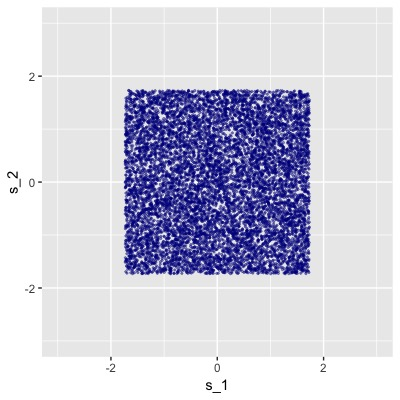
\includegraphics[width=5cm]{unif-plot.jpeg}
			\caption{two independent uniformly distributed random variables}
			\label{unif-plot}
		\end{minipage}
		\hfill
		\begin{minipage}[hbt]{7cm}
			\centering
			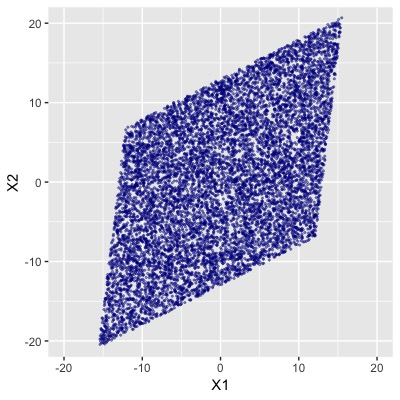
\includegraphics[width=5cm]{unif-mixed-plot.jpeg}
			\caption{mixtures of two uniformly distributed random variables}
			\label{unif-mix-plot}
		\end{minipage}
	\end{figure}
	
	The following example relies on \citet{ICA_Book}.
	Assume we have two independent components $S_1$ and $S_2$ which have the following uniform distribution:
	\begin{equation}
	p(S_i)=\begin{cases} \frac{1}{2 \sqrt {3}} &\text{if $\vert S_i \vert \leq \sqrt{3}$}\\
	0 &\text{otherwise.}
	\end{cases}
	\end{equation}
	We choose this distribution so our two independent components have zero mean and unit variance.
	In figure \ref{unif-plot} we see \mbox{$(2 \times 10000)$} data points drawn from this distribution.
	Because of our choice of $p$ the points form a cuboid.
	
	Then we mix these variables with the mixing matrix
	\begin{equation}
	A=
	\begin{pmatrix}
	1 & 8 \\
	8 & 4
	\end{pmatrix}
	\end{equation}
	to get our observable data \mbox{$X_1$} and \mbox{$X_2$}.
	As we can see in figure \ref{unif-mix-plot} the mixtures now form a parallelogram. (Note that figure \ref{unif-mix-plot} is larger scaled than figure \ref{unif-plot}.)
	After the mixing process the two components are no longer independent.
	By choosing \mbox{$X_1$} in the upper right corner of the parallelogram we already determine the value for \mbox{$X_2$}.
	This leads us to the assumption that we gain informations about the mixing matrix $A$ if we look in the edges.
	The shift of the edges gives us the directions of the columns of our mixing matrix $A$.
	In fact we can estimate our ICA model by first estimating the joint density of \mbox{$X_1$} and \mbox{$X_2$} and then locating the edges.
	
	
	
	Given the mixed signal samples $X$,  ICA algorithms now try to obtain a \textit{demixing matrix} $W$ that recovers the original source signal $S$. The demixed signal $V$ is now given by:
	\begin{equation}
	V = WX
	\end{equation}
	
	We know that we found the ideal solution \mbox{($V = S$)} if the equation \mbox{$W=A^{-1}$} holds.
	According to \citet{estimating-smi-ica} we can only recover the setup up to permutation and scaling of components of $S$. 
	And we have the same problem of ambiguity that we already had in chapter \ref{factoranalysis}.\\ %Insert explanation: adding a matrix S and getting a "new" A
	
	%way more information needed, paragraph of the main topic is too short!
	%add another paragraph about the difference to other algorithms/find out what it has to do with the independent S_l
	\begin{minipage}{\textwidth}
		As we already discussed in section \ref{cocktailparty} we need assumptions on \mbox{$S, X$} and \mbox{$A$} to make the problem more unique. According to \citet{ICA_Book} these assumptions are:
		\begin{enumerate}
			\item The independent components $S_i$, $ i=1,\dots,p$ are statistically independent.
			\item The independent components $S_i$, $ i=1,\dots,p$ must have non-Gaussian \linebreak distributions
			\item For simplicity, we assume the unknown mixing matrix $A$ to be square.
		\end{enumerate}
	\end{minipage}\\~\\
	
	%Var(S)=I (unit variance) else: problem with ambiguity
	
	The first point is the principal assumption we need for ICA and we do not need much more to assure that our problem can be estimated.
	This makes ICA to a very powerful and versatile tool.
	%example what happens with two variables that depend on each other; maybe it doesnt fit here
	If we try to estimate to dependent variables, we can no longer use ICA.
	Let us for example assume two uniform distributed variables \mbox{$\tilde{S_1}$} and \mbox{$\tilde{S_2}$} that are no longer independent.
	They could look like in figure \ref{unif-mix-plot}.
	So let us assume that these \mbox{$\tilde{S_i}$} are orthogonal transformed via the matrix \mbox{$A_0$} and two uniform distributed independent components \mbox{$S_1$} and \mbox{$S_2$}.
	As a next step we mix these sources (again) using an orthogonal matrix \mbox{$\tilde{A}$}.
	But what happens if we try to estimate our new observations \mbox{$X=\tilde{A}\tilde{S}$} with ICA?
	Using that the \mbox{$\tilde{S_i}$} are also mixtures we get: \mbox{$X=\tilde{A}A_0S$}.
	By writing \mbox{$R=\tilde{A}A_0$} we get the orthogonal matrix $R$ that describes how the independent components are mixed to get our observations $X$.
	So if we apply our ICA algorithm we get the sources \mbox{$S_1$} and \mbox{$S_2$} and not the dependent variables \mbox{$\tilde{S_1}$} and \mbox{$\tilde{S_2}$}.
	
	The second point is the main difference between ICA and other models that estimate linear mixed components.
	The non-Gaussianity will be discussed in chapter \ref{ica:clt}.
	
	The last point is equivalent to saying that the number of independent components is the same as the number of observed mixtures.
	In our cocktail party problem from section \ref{cocktailparty} this is equivalent to having the same number of microphones and speakers.
	%what happens without this assumption/what exactly do we need it for ->MAYBE: otherwise the problem is still underparametrized
	
	\subsection{Theoretical background} \label{ica:basics}
	
	%Maybe the central limit theorem suits here: explain why we want non-Gaussianity
	
	The following subsection relies on \citet{elementsofstatisticallearning} and \citet{ICA_Book}.
	
	Without loss of generality we assume $X$ to be whitened.
	
	According to \citet{ICA_Book} this means:
	
	\begin{Definition}
		A zero mean vector $z=(z_1,\dots,z_n)^T$ is said to be \normalfont{white} \textit{if its elements $z_i$ are uncorrelated and have unit variances: $E(z_iz_j)=\delta_{ij}$.}
	\end{Definition}
	
	We can also state that \mbox{$Cov(S)=I$} because the \mbox{$S_i$, $ i=1,\dots,p$} are independent and as a consequence uncorrelated. %insert: A proof can be found for example in ..
	There could now be values that are not equal to $1$ on the diagonal of the matrix but we can still assume that $S$ has the covariance matrix $I$.
	This is because we can just put the variances of the \mbox{$S_i$, $i=1,\dots,p$} into the matrix $A$. %not sure about this part
	
	From the assumptions that $X$ is whitened and the $S_i$ are independent it follows that $A$ is orthogonal:
	\begin{equation}\label{orthogonality}
	I=Cov(X)=Cov(AS)=ACov(S)A^T=AA^T.
	\end{equation}
	And instead of having to estimate $n^2$ parameters of our mixing matrix we only need to estimate \mbox{$\frac{n(n-1)}{2}$} parameters by restricting the matrix $A$ to the subspace of orthogonal matrices. %maybe source for the numbers
	There are many different preprocessing algorithms to whiten a random variable that are for example discussed in \citet{ICA_Book}
	and it is a transformation that is possible for all random variables. (In other words: it does not need any additional assumptions.)
	%In addition we can easily reconstruct the mixing matrix $\tilde{A}$ of our untreated random variable $\tilde{X}$.
	In addition whitening is computationally very simple and a standard procedure that helps to reduce the complexity of our problem.
	This is why it is useful for us to pre-whiten our mixed signal $X$ before we start with the algorithm.
	
	
	\subsubsection{The central limit theorem -- Why do we want non-gaussianity} \label{ica:clt}
	%maybe dont make it a paragraph, could also fit directly after the first assumptions
	Our second assumption in section \ref{ica} says, that we want our independent component to be non-Gaussian.
	The central limit theorem is a very important result in statistics and it helps us to understand why we need our variable $S$ to be non-Gaussian or at least as non-Gaussian as possible. According to \citet{wtheorie}
	the central limit theorem is defined in the following way:
	\begin{Theorem}
		Let \mbox{$X_1,X_2,\dots$} be independent identically distributed real valued random variables with \mbox{$\mu := E\left(X_1\right) \in \mathbb{R}$} and \mbox{$\sigma^2 := Var\left(X_1\right) \in \left(0,\infty\right)$}. For \mbox{$n \in \mathbb{N}$} set \mbox{$S^*_n := \frac{1}{\sqrt{\sigma^2n}}\sum_{i=1}^{n}\left(X_i-\mu\right)$}. Then
		\begin{equation}
		P_{S^*_n} \xrightarrow{\enskip n \to \infty \enskip} N_{0,1} \text{ weakly.}
		\end{equation}
	\end{Theorem}
	%state the reason
	In summary it says that if we are looking at the standardized sum of independent random variables, their distribution tends towards a Gaussian distribution.
	
	The following example relies on \citet{ICA_Book}.
	To understand why we want non-Gaussianity, we discuss what happens if we have two variables \mbox{$s_1$} and \mbox{$s_2$} that have a Gaussian joint distribution.
	This distribution has the form:
	\begin{equation}
	p(s_1,s_2)=\frac{1}{2\pi} \exp \left(-\frac{s_1^2+s_2^2}{2}\right)=\frac{1}{2\pi}\exp \left(-\frac{\vert \vert s \vert \vert ^2}{2}\right)
	\end{equation}
	The equation \mbox{$X=AS$} then leads us to the density of the mixtures \mbox{$x_1$} and \mbox{$x_2$}:
	\begin{equation}
	p(x_1,x_2)=\frac{1}{2\pi}\exp \left(-\frac{\vert \vert A^T x \vert \vert ^2}{2}\right)\vert \det A^T \vert 
	\end{equation}
	As we have already shown in equation \ref{orthogonality}, our mixing matrix $A$ is orthogonal and as a consequence \mbox{$A^{-1}=A^T$}.
	We now use this fact to simplify the density.
	Orthogonal transformation is norm invariant, which leads to \mbox{$\vert \vert A^T x \vert \vert ^2 = \vert \vert x\vert \vert ^2$}.
	For an orthogonal matrix we also know that \mbox{$\vert \det A \vert = 1 $} holds.
	This leads us to the following density:
	\begin{equation}
	p(x_1,x_2)=\frac{1}{2\pi}\exp \left(-\frac{\vert \vert x \vert \vert ^2}{2}\right).
	\end{equation}
	The density does no longer contain the orthogonal matrix $A$ and therefore the mixing does not change the product density function.
	Actually the original and the mixed signals have exactly the same distribution.
	As a result we can not estimate the mixing matrix $A$ if we have two Gaussian variables.
	It is easy to see that we get the same problem with more than two Gaussian variables.
	For our model this means hat we can not deal with more than one Gaussian variable.
	
	\begin{figure}[hbt]
		\begin{centering}
			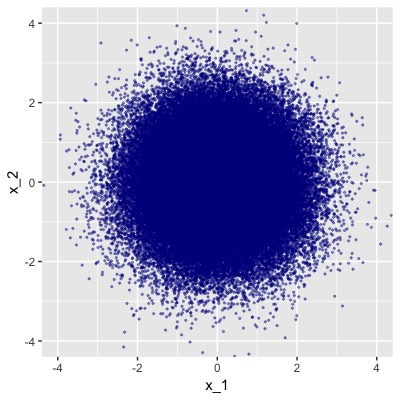
\includegraphics[width=5cm]{gauss-plot.jpeg}
			\caption{Two gaussian variables $x_1$ and $x_2$}
			\label{gauss-plot}
		\end{centering}
	\end{figure}
	Alternatively we can also observe this phenomenon graphically.
	In figure \ref{gauss-plot}
	we can see, that if we rotate the distribution it will look the same as before (the distribution is rotationally symmetric).
	So there are no informations about the directions of the columns of $A$ in our density and we can not estimate the mixing matrix.
	
	\subsubsection{The kurtosis -- measuring non-gaussianity} \label{kurtosis}
	
	The following paragraph relies on \citet{ICA_Book}. 
	
	In the previous section we found out that we want our vectors \mbox{$S_i$} to be as non-Gaussian as possible.
	Now we define how we can measure this non-Gaussianity.
	
	In many approaches higher order cumulants are used as a measure.
	
	Given a random variable $X$ the first four cumulants are:
	\begin{equation}
	\begin{split}
	k_1 &= E(X)\\
	k_2 &= E(X^2)-(E(X))^2\\
	k_3 &= E(X^3)-3E(X^2)E(X)+2(E(X))^3\\
	k_4 &= E(X^4)-3(E(X^2))^2-4E(X^3)E(X)+12E(X^2)(E(X))^2-6(E(X))^4
	\end{split}
	\end{equation}
	
	If the random variable $X$ has zero mean, the first four cumulants simplify to
	\begin{equation}
	\begin{split}
	k_1 &= E(X)\\
	k_2 &= E(X^2)\\
	k_3 &= E(X^3)\\
	k_4 &= E(X^4)-3(E(X^2))^2
	\end{split}
	\end{equation}
	As we can see, the first three cumulants are equal to the respective moments.
	
	%change sentence for Transition
	The normalized version of the fourth moment, called \textit{kurtosis} ist often applied in ICA algorithms to measure non-Gaussianity.
	
	If $X$ is a zero mean random variable the kurtosis is defined as
	\begin{equation}
	\kurt (X) = E(X^4)-3(E(X^2))^2.
	\end{equation}
	Which in fact equals the fourth moment of a zero mean variable.
	We can now normalize the kurtosis with respect to the variance and get:
	\begin{equation}
	\tilde{k}(X) = \frac{E(X^4)}{(E(X^2))^2}-3.
	\end{equation}
	%where does the normalized version come from?
	If the data is additionally whitened, which means that the variance is normalized %?
	\mbox{($E(X^2)=1$)}, the kurtosis and the normalized version of kurtosis are equal:
	\begin{equation}
	\kurt (X) = E(X^4)-3 =\tilde{k}(X)
	\end{equation}
	
	The kurtosis has some usefull propertys.
	The first important feature is its additivity: given any statistically independent random variables $X$ and $Y$ the kurtosis of the sum equals the sum of the kurtosis:
	\begin{equation}
	\kurt (X+Y)= \kurt (X)+\kurt (Y)
	\end{equation}
	But its not a linear function. Because given any scalar \mbox{$\beta$}
	\begin{equation}
	\kurt(\beta X) = \beta^4 \kurt(X)
	\end{equation}
	%following paragraph is the most relevant part/main thesis i will need later. Maybe shorten the part above?
	The kurtosis also indicates non-Gaussianity. If $X$ is a Gaussian variable it follows that \mbox{$\kurt(X) = 0$}.
	This simply relies on the normalisation as described above.
	So if we want a random variable that is a far from Gaussian as possible we want \mbox{$\kurt(X)$} to be as far from zero as possible.
	There are in general two possibilities to achieve this goal: the kurtosis could be very big or it could be very small.
	If \mbox{$\kurt(X)>0$} the respective distribution is called \textit{supergaussian}.
	The corresponding graph has a sharper peak and longer tails than the Gaussian distribution.
	It is also not limited to the top, the kurtosis can strive after infinite.
	If \mbox{$\kurt(X)<0$} the respective distribution is called \textit{subgaussian}.
	The corresponding graph is flatter than the Gaussian distribution and has heavier tails.
	As opposed to the supergaussian distribution, the kurtosis of the subgaussian distribution is limited.
	It can not get below \mbox{$-2$}.
	Before we proof this limitation we repeat an important theorem in mathematics which can for example be found in \citet{wtheorie} :
	\begin{Theorem} \label{hoelder-theorem} \textbf{(Hölder's inequality)}
		For $p,q$ $\in \left[ 1,\infty\right]$ with $\frac{1}{p}+\frac{1}{q}=1$ and $f \in L^p(\mu)$, $g \in L^q(\mu)$ it holds that $(fg) \in L^1(\mu)$ and
		\begin{equation}\label{hoelder-inequality}
		\vert \vert fg \vert \vert _1 \leq \vert \vert f \vert \vert _p \vert \vert g \vert \vert _q.
		\end{equation}
	\end{Theorem}
	Where \mbox{$L^p(\mu)$} indicates the aggregate of all functions for which \mbox{$\vert \vert f \vert \vert _p < \infty$} holds.
	
	But how does this theorem help us to show the lower border of \mbox{$\kurt(X)$}?
	Let us try to restate our assumption:
	\begin{equation}\label{estimate-kurt}
	\begin{split}
	-2& \leq \kurt(X) \\
	\Leftrightarrow -2 & \leq E(X^4) -3\\
	\Leftrightarrow 1 & \leq E(X^4).
	\end{split}
	\end{equation}
	%Now we use that $x$ is white and that the variance of the variable equals $1$ to get:
	%\begin{equation} \label{fourthmomentinequality}
	%E(X^4) \geq  E(X^2).
	%\end{equation}
	As a next step we try to modify theorem \ref{hoelder-theorem} so that it helps us to show equation \ref{estimate-kurt}.
	%If $p,q \in \left[ 1, \infty \right)$ we can write the respective norms as 
	%\begin{equation}
	%\left( \int \vert f \vert ^p d\mu \right)^{\frac{1}{p}}  \text{and} \left( \int \vert g \vert ^q d\mu \right)^{\frac{1}{q}}
	%\end{equation}
	For the probability space \mbox{$\left( \Omega, F, \mathbb{P}\right)$} and the expectation \mbox{$E(.)$} we can write \ref{hoelder-inequality} as
	\begin{equation}
	E\left(\vert XY\vert \right) \leq \left( E\left(\vert X \vert ^p \right)\right)^{\frac{1}{p}}\left( E\left(\vert Y \vert ^q \right)\right)^{\frac{1}{q}}.
	\end{equation}
	Now we choose \mbox{$Y = 1_{\Omega}$}, \mbox{$X=X^2$} and set \mbox{$p=\frac{n}{m}$} with \mbox{$n=4$} and \mbox{$m=2$}.
	We receive:
	\begin{equation}
	E(X^2) \leq \left(E\left(X^4\right)\right)^{\frac{1}{2}}.
	\end{equation}
	We are looking at the expectation of positive values so we can square both sides without violating the inequality.
	
	And now we get the estimation for the fourth moment that we want:
	\begin{equation}
	1 = \left( E(X^2) \right) ^2 \leq E\left(X^4\right).
	\end{equation}
	Therefore we proofed that the lower bound of kurtosis is $-2$.
	
	Because of the missing symmetry of kurtosis it is not possible to compare two random variables if one has a kurtosis smaller than zero and one has a kurtosis greater than zero.
	We can only compare two random variables if the corresponding kurtosis have the same sign. %is sign the right translation? what means that kurtosis is not the best method to compare if a random variable is less Gaussian -> need something else
	
	So in fact kurtosis is not always a good measure for non-Gaussianity and we need a different approach.
	An other measure that is often used in ICA is \textit{negentropy} which we will discuss in the next chapter.
	
	\subsubsection{Entropy and negentropy} \label{entropy}
	
	The following section relies on \citet{ICA_Book}.
	
	The basic concept of information theory is entropy.
	It is often used as a measure of \textit{randomness}.
	
	Let \mbox{$X$} be a discrete valued random variable. Then its entropy \mbox{$H$} is defined as
	\begin{equation}
	H(X)=-\sum_i P(X=a_i) \log P(X=a_i)
	\end{equation}
	where \mbox{$a_i$} are possible values for \mbox{$X$}. In other words the \mbox{$a_i$} are all elements of the state space%is this the right term?  %find better explanation fo the a_i/entropy in general
	%entropy: regularization measure/ measure of randomness
	The entropy of a random variable can be seen as the amount of information that the observation of the variable gives.
	The more unstructured and unpredictable a variable is, the larger its entropy. 
	If the entropy is very small it is more likely that the random variable takes a special value. %large entropy -> cannot predict value, small entropy -> a special value is much more likely than any other value
	%EXAMPLES!
	
	The following two examples rely on \citet{ICA_Book} and illustrate the different cases.
	
	%continous valued random variable: differential entropy, generalized
	The differential entropy \mbox{$H$} of a random variable \mbox{$X$} with density \mbox{$p_X(.)$} is defined as:
	\begin{equation}
	H(X)= - \int p_X(\xi) \log p_X(\xi) d\xi
	\end{equation}
	and can be interpreted in the same way as the discrete entropy.
	%interpreted as measure of randomness in the same way as entropy
	%maybe mutual information
	If we want to compare the amount of information two (or more) random variables contain, we use \textit{mutual information}. It is a measure of the information that members of a set of random variables have on the other variables in the set.
	
	The mutual information \mbox{$I$} between \mbox{$n$} scalar random variables \mbox{$X_i$, $ i=1,\dots,n$} is defined as:
	\begin{equation}
	I(X_1,\dots,X_n)=\sum_{i=1}^{n}H(X_i)-H(X)
	\end{equation}
	where $X$ is the vector containing all the \mbox{$X_i$}.
	
	One fundamental result in information theory and in applying entropy is that the Gaussian distribution is the most random and least structured of all distributions.
	
	As a result we can modify entropy to get a measure of non-Gaussianity.
	
	This leads us to \textit{negentropy} a measure that describes the distance between the entropy of a Gaussian random variable and an other random variable.
	The definition of negentropy $J$ is now very intuitive:
	\begin{equation}
	J(X) = H(X_{gauss})-H(X)
	\end{equation}
	where \mbox{$X_{gauss}$} is a Gaussian random vector of the same covariance matrix as $X$. %State in one sentence what exactly negentropy measures. Somethin like: increase information? Doesn´t realy make sense..
	Negentropy is always nonnegative. (because a Gaussian random variable has the highest entropy)
	If $X$ is Gaussian the variable \mbox{$X_{gauss}$} with Gaussian
	distribution and the same covariance matrix equals $X$ itself
	and as a result the negentropy is \mbox{$J(X)=0$}.
	Negentropy is also scale invariant \mbox{($J(aX)=J(X)$)}.%why
	
	Since negentropy and entropy both are not easy to compute
	we need approximations to apply these measurements.
	Details can be found in \citet{ICA_Book}.
	
	\subsection{Algorithm} \label{ica:algorithm}
	Returning to the ICA algorithm, we will now use the theoretical insights of chapter \ref{ica:basics} to formulate a concrete approach and a derivation of an ICA algorithm.
	
	\subsubsection{Product density ICA --  A direct approach}\label{ica:approach}
	%Maybe add the example from the ICA Book to show the part about the product density (Illustration of ICA, page 155)
	The following part %maybe theres a better word
	relies on \citet{elementsofstatisticallearning}.
	%go through the book (after writing the first points on my own) and look for additional information
	% In the following Paragraph the Problem ist to solve X=AS
	
	For the direct approach to ICA we use the assumption that the \mbox{$S_j$} are independent so that the joint density equals the product density:
	\begin{equation}
	f_S(s)=\prod_{j=1}^{p}f_j(s_j)
	\end{equation}
	In the following algorithm we will see that this approach estimates the density above directly using generalized additive models, that we have already discussed in chapter \ref{additivemodels}.
	
	The \mbox{$X_j$} are supposed to be as far from Gaussian as possible.
	To achieve this we want to represent the departures from the Gaussian distribution. 
	In chapter \ref{entropy} we already discussed the measure negentropy which we will use to satisfy our constraint.
	We now define each density \mbox{$f_j$} for the component \mbox{$S_j$} as:
	\begin{equation}\label{tilted-gaussian}
	f_j(s_j)=\phi (s_j)e^{g_j(s_j)}
	\end{equation}
	so that each \mbox{$f_j$} is a tilted Gaussian density (\mbox{$\phi(.)$} is the standard gaussian density) and we choose the \mbox{$g_j$} in order that \mbox{$f_j$} satisfies the normalization conditions of a density. %maybe add examples for g
	%do we use the clt here? Because we can estimate the densitys with a tilted gaussian. Is there a connection to 
	As before we assume $X$ to be pre-whitened.
	
	As a next step we look at the log-likelihood function of the observed data \mbox{$X=AS$}:
	\begin{equation}
	l(A,\{g_j\}_1^p;X)=\sum_{i=1}^N \sum_{j=1}^p [\log \phi_j (a_j^T x_i) + g_j(a_j^Tx_i)]
	\end{equation}
	%In a different source the sums are Integrals, maybe make a short sentence why they are equivalent
	Now we want to maximize this function, provided that $A$ is orthogonal and the \mbox{$g_j$} are chosen in a way that \mbox{$f_j$} is a density.
	
	This problem is over-parametrized. So we maximize a regularized version instead that already includes our restrictions on $A$ and the \mbox{$g_j$}:
	\begin{equation}
	\sum_{j=1}^p[\frac{1}{N}\sum_{i=1}^N[\log\phi(a_j^Tx_i)+g_j(a_j^Tx_i)]-\int\phi(t)e^{g_j(t)}dt-\lambda_j\int\{g_j^{\prime\prime\prime}(t)\}^2(t)dt].
	\end{equation}
	In this regularized function two penalty terms are substracted. The first one makes sure, that the density constraint
	\begin{equation}
	\int \phi (t)e^{\hat{g}_j(t)}dt = 1
	\end{equation}
	is satisfied for any possible solution \mbox{$\hat{g}_j$}.
	The second integral is a roughness penalty. It guarantees that any solution \mbox{$\hat{g}_j$} is a quartic-spline with knots at the observed values of \mbox{$s_{ij}=a_j^Tx_i$}. %why do i want these splines?
	
	This leads to the following definition of the Product Density ICA algorithm:\\
	
	%check if Algorithm is translated correctly
	\begin{minipage}{\textwidth}
		\begin{Algorithm} \label{Algorithm}
			\hspace{0.5cm}
			\begin{enumerate}
				\item Initialize A as a Gaussian random matrix with subsequent orthogonalization
				\item Alternate until convergence of A:
				\begin{enumerate}
					\item Given A, optimize
					\begin{equation}\label{ProDenICAalg}
					\sum_{j=1}^p[\frac 1 N \sum_{i=1}^N[\log\phi(a_j^Tx_i)+g_j(a_j^Tx_i)]-\int\phi(t)e^{g_j(t)}dt - \lambda_j\int\{g_j^{\prime\prime\prime}(t)\}^2(t)dt].
					\end{equation}
					with respect to \mbox{$g_j$} and for each $j$ separately.
					\item Given \mbox{$g_j, j = 1, \dots, p$}, make one step of a fixed point algorithm to find a better matrix A.
				\end{enumerate}
			\end{enumerate}
		\end{Algorithm}
	\end{minipage}\\~\\
	
	% talk about the fixed point algorithms that can be used and that are most frequently used (?)
	
	In summary, the algorithm fits the functions \mbox{$g_j$} and the directions \mbox{$a_j$} by alternating the optimization of function \ref{ProDenICAalg}.
	
	The resulting densities \mbox{$\hat{f}_j=\phi \exp ^{\hat{g}_j}$} have zero mean and variance one. %maybe add proof, in elements of statistical learning its exercise 14.18 on page 582
	If we increase the \mbox{$\lambda_j$} in function \ref{ProDenICAalg} our solutions tend towards the standard gaussian distribution \mbox{$\phi$}.
	
	To check if we estimated the mixing matrix $A$ good enough, we use the \textit{Amari metric}.
	It is a measure for the closeness of two frames.
	Given the real orthogonal mixing matrix \mbox{$A_0$} this metric is defined as:
	\begin{equation}
	d(A_0,A)=\frac{1}{2p}\sum_{i=1}^{p}\left( \frac{\sum_{j=1}^{p} \vert r_{ij} \vert}{max_j \vert r_{ij} \vert}-1 \right) +\frac{1}{2p}\sum_{j=1}^{p}\left( \frac{\sum_{i=1}^{p} \vert r_{ij} \vert}{max_i \vert r_{ij} \vert}-1\right)
	\end{equation}
	where \mbox{$r_{ij}=(A_0A^{-1})_{ij}$}.
	
	\subsubsection{Convergence} \label{ica:convergence}%maybe, if its not too much. Look through the papers you printed for the seminar, there was a phd thesis about this. Maybe parts of it are relevant
	%maybe dont make it a chapter on its own or change it to "Why does this algorithm work properly" and dont realy go deep into a proof of convergence
	
	\subsection{Comparison of different ICA algorithms}
	%"Estimating Square-.loss Mutual Information for Independent Component Analysis" from Taiji Suzuki ans Masashi Sugiyama could be a good source for this chapter
	\newpage
	
	\section{Implementation} 
	In the following section the ICA algorithm is used for ... %add what type of data will be observed
	in R.
	%time-series seem to be an interesting application, maybe kryptocurrency data prediciton? -> Check if there is already any implementation in R, maybe talk to Mr. Müller -> timeseries, baysian statistics..., try to remember where the krypto-data came from/how you were able to export it
	%Alternative: Use FastICA (Book) as in the Seminar, just showing the errors with different distributions. (last option, kind of boring)
	%Maybe there is even an alternative Dataset for an useful Implementation/usage of the FastICA Package, maybe even related to the Cocktailparty-Problem
	\subsection{The ProDenICA Package}
	The package \textit{ProDenICA} is an implementation of the
	direct approach described in section \ref{ica:approach}.
	For the detailed package documentation see \citet{prodenica-doku}.
	
	It includes various functions that are needed to prepare the given data,
	e.g. \textit{ICAorthW} that is used to turn a matrix W into an orthogonal matrix by computing its singular value decomposition. %how exactly is the orthogonal matrix achieved
	The package also provides a function called \textit{mixmat} to generate
	a random mixing matrix of a given dimension with condition number %right term?
	between 1 and 2, so that we have a matrix to start with algorithm \ref{Algorithm}.
	Besides it includes a function to compute the amari metric that allows us to analyze the correctness of the ICA algorithm.
	
	Further explanations and examples are found in the Package description \citep{prodenica-doku}
	
	\subsection{Example with generated data}
	
	The ProDenICA package gives an example how to generate source signals using the tilted gaussian distribution described in equation \ref{tilted-gaussian}.
	It has 18 %(?)
	different functions for \mbox{$g(.)$}. %plot the different distributions(!)
	
	Once again we assume two source signals \mbox{$S_1$} and \mbox{$S_2$} and join them in a matrix $S$.
	Then we generate a random mixing matrix $A$ with condition number between $2$ and $3$ %check number
	using the function mixmat.
	To compare the result of the algorithm afterwards we also compute the inverse $A^{-1}$ of $A$.
	For the mixing process we simply multiply \mbox{$X=AS$}.
	Afterwards we whiten the generated observation $X$ as described in ... %describe whitening process and reference it here
	Before we start with the algorithm we need to set the starting point for the iteration.
	We choose a random matrix \mbox{$W_0$} that has gaussian entries and orthogonalize it afterwards with the function \textit{ICAorthW} from the package ProDenICA.
	After these preprocessing steps we start the main part of the algorithm.
	
	
	\subsection{Example with real life data}
	\subsubsection{How the Data is used}
	Now we want to use this package to apply the algorithm to a variation of the cocktail party problem.
	We take two individually recorded sounds, \mbox{$S_1$} and \mbox{$S_2$}, and mix them with a random mixing matrix \mbox{$\hat{A}$}.
	Such a matrix can be computed with the R function mixmat. %maybe explain mixmat a bit: a <- matrix(rnorm(p*p),p,p); sa <- svd(a); d <- sort(runif(p)+1); mat <- sa$u %*% (sa$v * d); attr(mat, "condition") <- d[p]/d[1]; mat
	By taking this step we make it easier to see if our algorithm works properly. %maybe other words, by mixing the sounds with a known matrix/...
	By mixing the original sources we get two mixed signals \mbox{$X_1$} and \mbox{$X_2$}, that we will be trying to separate in the following part.
	%Explain the data a bit: first row is is this sound, second is that sound..
	
	At first we want to whiten our observed data.
	We need this step because all of our assumptions rely on the fact that the observations $X$ are whitened.
	Theoretically this can be achieved with the R function scale.
	This function takes a vector, substracts the mean and divides it by the standard deviation.
	But it does not keep the factors by which it scales our data.
	To be able to invert the scaling later we have to make these steps manually. %add a little "why do we want to rescale" and how exactly are we scaling/maybe check if the matrix actually is white afterwards.
	As a next step we compute the singular value decomposition of \mbox{$X=UDV^T$} and scale the vector in the following way:
	\begin{equation}
	X=\sqrt{N}U
	\end{equation}
	where $N$ is the number of observations.
	
	\subsubsection{What is the Outcome}
	%make fancy graphics about the results/resulting data of the implementation
	After finding the mixing matrix $A$ we can compare the result of our algorithm with the real mixing matrix \mbox{$\hat{A}$} and the resulting source signals \mbox{$S_1$} and \mbox{$S_2$} with the actual sources \mbox{$\hat{S_1}$} and \mbox{$\hat{S_2}$}.
	
	\newpage
	\section {Conclusion}
	%summarize advantages and disadvantages of ICA; Write something about its applications and that there are still many researches in this field/future of machine learning and/or unsupervides learning algorithms; is it funny to end with a statement about machines being more intelligent than humans?
	%could also contain something about 
	\newpage
	
	\thispagestyle{plain}
	\bibliographystyle{chicago}%does not work completely yet
	\bibliography{bareference}
	
\end{document}